
% !TEX root = NotesDeCours.tex


\part{Chapitre 10 : Acoustique}

% ================================================================================================ 
% Page de titre :
% ================================================================================================

\begin{frame}

  \color{bleu}

  \begin{flushleft}
    
    \Large
   	\bf
    
    Mécanique des fluides 

  \end{flushleft}
  
  \ligne{3} % remplace: \noindent \thickline{0.5mm}{150}

  \begin{flushright}

    \rm

    \textrm{David} \textsc{Fabre}
    
    \vspace{3mm}
    
    IMFT / UPS
    
    Département de Mécanique
    
%    brancher@imft.fr

  \end{flushright}

\begin{picture}(110, 40)(0, 0)
  \put( 0,  0){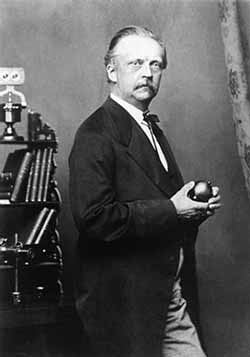
\includegraphics[height=47mm]{helmholtz.jpg}}
  \put(34,  0){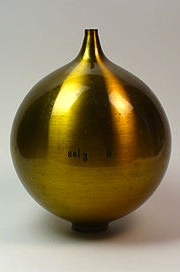
\includegraphics[height=47mm]{resonator_crop.jpg}}
  \put(67, 8.5){\color{gris} \small \rm 
  	\begin{minipage}{38mm}
  		Hermann Ludwig Ferdinand \\ von Helmholtz (1821--1894)
		\\ tenant dans ses mains \\ le résonateur
		acoustique \\ qui porte son nom, \\ photographié ci-contre.
	\end{minipage}}
\end{picture}

  \vspace{5mm}
  
  \begin{flushright}
    
    \Large
   	\bf
    
    %\sout{11.} 
    \quad  10. Acoustique

  \end{flushright}

  \vspace{7mm}

\end{frame}

%%%%%%%%%%%%%%%%%%%%%%%%%%%%%%%%%%%%%%%%%%%%%%%%%%%%%%%%%%%%%%%%%%%%%%%%%%%%%%%%%%%%%%%%%%
% Sommaire :
%%%%%%%%%%%%%%%%%%%%%%%%%%%%%%%%%%%%%%%%%%%%%%%%%%%%%%%%%%%%%%%%%%%%%%%%%%%%%%%%%%%%%%%%%%

\begin{frame}{Sommaire}

\small
  
\hspace*{2mm}
\begin{tabular}{cc}
		%&
  		\begin{minipage}{62mm}
  			\tableofcontents[firstsection=-8]
      \vspace{15mm}
  		\end{minipage}
  		&   
  		\begin{minipage}{60cm}
		  \vspace*{-5mm}  
  			%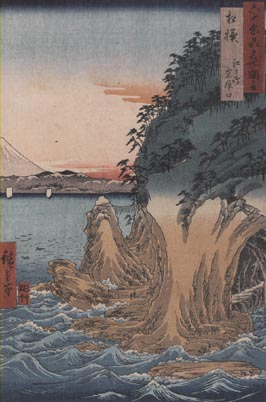
\includegraphics[width=40mm]{vagues.jpg} 
  		\end{minipage}
  	\end{tabular}

\vspace{0mm}

\end{frame}

%%%%%%%%%%%%%%%%%%%%%%%%%%%%%%%%%%%%%%%%%%%%%%%%%%%%%%%%%%%%%%%%%%%%%%%%%%%%%%%%%%%%%%%%%%
\section{\bfseries Acoustique}
%%%%%%%%%%%%%%%%%%%%%%%%%%%%%%%%%%%%%%%%%%%%%%%%%%%%%%%%%%%%%%%%%%%%%%%%%%%%%%%%%%%%%%%%%%
%==========================================================================================
\subsection{Equations de l'acoustique}
%=========================================================================================

%-----------------------------------------------------------------------------------------
\subsubsection{Cadre de la modélisation}
%-----------------------------------------------------------------------------------------
\begin{frame}{Cadre de la modélisation}
%-----------------------------------------------------------------------------------------

\small

\pause

\textbf{Cadre :} \medskip

état de base : fluide au repos
\[
	\myvec{u}_0 = \myvec{0}
\]
et grandeurs thermodynamiques uniformes (pas de variation spatiale) 
\[
	p=p_0, \quad T=T_0, \quad \rho = \rho_0
\]

Gravité négligée.

\bigskip \pause

\textbf{Objectif :} \medskip

déterminer l'évolution de perturbations de cet état de base :
\[
	\myvec{u} = \myvec{u}_0 + \myvec{u}\myprime(\myvec{x}, t), \quad
  p = p_0 + p\myprime(\myvec{x}, t), \quad
  T = T_0 + T\myprime(\myvec{x}, t), \quad
  \rho = \rho_0 + \rho\myprime(\myvec{x}, t)
\]

\bigskip \pause

\textbf{Hypothèses :} \medskip

on supposera ces perturbations "petites" (ou infinitésimales), d'ordre $\varepsilon \ll 1$
\[
	\frac{p\myprime}{p_0}, \; \frac{T\myprime}{T_0}, \; \frac{\rho\myprime}{\rho_0}, 
	\; 
	\frac{\myvec{u}\myprime}{c_0}
	\sim \varepsilon \ll 1	
\]

Remarque : la seule échelle de vitesse est $c_0 = 1/\sqrt{\rho_0 \chi_s}$.

\smallskip 
Echelle de temps associée : $\tau_{ac} =  L/c_0$ 


\vspace{10mm}

\end{frame}

%-----------------------------------------------------------------------------------------
\subsubsection{Equation de la quantité de mouvement}
%-----------------------------------------------------------------------------------------
\begin{frame}{Conservation de la quantité de mouvement : Analyse dimensionnelle}
%-----------------------------------------------------------------------------------------

\small

Equation locale de bilan de quantité de mouvement (cf. chapitre 5) :
\begin{equation}
\begin{array}{ccccccc}
\underbrace{\rho \dpdt{\myvec{u}}}_{\color{green}{[I]}} 
&+& 
\underbrace{\rho (\mytensor{grad} \myvec{u} ) \cdot \myvec{u}}_{\color{green}{[A]}} 
 &=&
\underbrace{ - \gradient p' }_{\color{green}{[P]}} 
 &+& 
 \underbrace{ \mu \left( \Delta \myvec{u} - \gradient (div(\myvec{u})/3)  \right)}_{\color{green}{[V]}} 
  \\
  \color{red}{\frac{\rho_0 [u']}{\tau_{ac}}}
  &&
   \color{red}{\frac{\rho_0 [u']^2}{L}}
&&
   \color{red}{\frac{[p']}{L}}
   &&
    \color{red}{\frac{\mu [u'] }{L^2}}
   \end{array}
\end{equation}

\pause

Régime Acoustique : le terme dominant est \textcolor{green}{[I]}.


\begin{itemize}
\item $\frac{[A]}{[I]}  \ll 1 \Longleftrightarrow \frac{[u']}{c_0} = Ma \ll 1$

\item $\frac{[V]}{[I]}  \ll 1 \Longleftrightarrow \frac{c_0 L}{\nu } = Ma / Re \ll 1$


{
\tiny
\color{gray}
(Remarque : Dans un gaz $\nu \approx v_q \ell$ où $\ell$ est le libre parcours moyen et $v_q$ la vitesse quadratique moyenne ($v_q \approx c_0$).
Donc $Ma / Re \approx L/\ell = Kn$. Le terme  visqueux est donc effectivement négligeable a partir du moment ou l'hypothèse du milieu continu est vérifiée !)
}
 


\item Le PMD permet de déterminer la jauge de pression $[p']$  : 
$\frac{[P]}{[I]}  \approx 1 \Longleftrightarrow \quad [p'] = \rho_0 [u'] c_0 $.
\end{itemize}


Sous ces hypothèses l'équation de Navier-Stokes se simplifie alors en :

$$
\color{vert}
\rho_0 \dpdt{\myvec{u}\myprime} = - \gradient p \myprime
$$

\end{frame}



%-----------------------------------------------------------------------------------------
\subsubsection{Equation de la masse}
%-----------------------------------------------------------------------------------------
\begin{frame}{Conservation de la masse : analyse dimensionnelle}
%-----------------------------------------------------------------------------------------

\small

Equation locale de bilan de masse (cf. chapitre 5) :
\begin{equation}
\begin{array}{cccccc}
   \underbrace{\dpdt{\rho}}_{\textcolor{green}{[I]}} 
   &+&
\underbrace{ \myvec{u} \cdot \gradient(\rho)}_{\textcolor{green}{[A]}}  
 &+& 
   \underbrace{\rho  \divergence (\myvec{u})}_{\textcolor{green}{[D]}}  
   &= 0 \\
    \color{red}{\frac{[\rho']}{\tau_{ac}}}
  &&
   \color{red}{\frac{[\rho'] [u']}{L}}
&&
   \color{red}{\frac{\rho_0[u']}{L}}
\end{array}   
\end{equation}

\pause \bigskip


Régime Acoustique : le terme dominant est \textcolor{green}{[I]}.


\begin{itemize}
\item $\frac{[A]}{[I]}  \ll 1 \Longleftrightarrow \frac{[u']}{c_0} = Ma \ll 1$

\item 
PMD : $\frac{[D]}{[I]} \approx 1$ 
$\Longrightarrow$ $\frac{[\rho']}{\rho_0}  = \frac{[u']}{c_0}$.
\end{itemize}



\bigskip \pause
L'équation linéarisée en perturbation s'écrit alors :
\begin{equation}
	\color{vert}
  \dpdt{\rho\myprime} + \rho_0 \divergence \myvec{u}\myprime = 0
\end{equation}

\vspace{5mm}

\end{frame}

%-----------------------------------------------------------------------------------------
\subsubsection{Compressibilité et vitesse du son}
%-----------------------------------------------------------------------------------------
\begin{frame}{Compressibilité : évolution thermodynamique}
%-----------------------------------------------------------------------------------------

\small

Equation-bilan de l'entropie massique $s$ (cf. MMC et Formulaire, annexe A)

\begin{equation}
		\rho T \ddt{s} 
		= \mytensor{\tau} : \mytensor{grad}(\vec{u}) - \divergence(\vec{q}). 
		%\label{eq:bilan_local_lagrangien_qdm}
\end{equation}

\pause

Si les mécanismes de diffusion (viscosité et conduction thermique) sont négligeables, l'évolution est {\color{red} isentropique }

$$
\ddt{s} = 0 
$$

\pause 

On peut alors (pour un gaz parfait) relier les variations de pression et de masse volumique par la loi de Laplace :

\smallskip
$$p\rho^{-\gamma} = cte$$ 

\pause

\smallskip
On en déduit :
$$
\frac{p'}{p_0} - \gamma \frac{\rho'}{\rho_0}  = 0
$$

Soit $p' = c_0^2 \rho'$ avec $c_0^2 = \frac{\gamma P_0}{\rho_0} = \gamma r T_0$


\medskip \pause
\textbf{Généralisation :}  

 $$
 c_0^2 = \frac{1}{\rho \chi_s} 
 $$ 
 
 où 
 $\chi_s = \frac{1}{\rho} {\left. \frac{\partial p}{\partial \rho} \right|}_s$ est le coefficient de compressibilité adiabatique.
 

\vspace{0mm}

\end{frame}


%-----------------------------------------------------------------------------------------
%\subsubsection{Vitesse du son}
%-----------------------------------------------------------------------------------------
\begin{frame}{Vitesse du son}
%-----------------------------------------------------------------------------------------

\small

%Les prédictions théoriques précédentes font apparaître la vitesse de propagation des ondes
%acoustiques, appelée vitesse du son, dont l'expression générale est donnée par

%Rappels : les propriétés thermodynamiques permettent de définir une échelle de vitesse, appelée vitesse du son, définie par

%\[
%	\color{vert}
%	c_0 = \dfrac{1}{\sqrt{\rho_0 \kappa_s}}
%\]	
%où $\rho_0$ désigne la masse volumique ambiante du fluide, supposée uniforme, 
%et $\kappa_s$ correspond \\ au coefficient de compressibilité isentropique du fluide
%dans les conditions thermodynamiques ambiantes.

%\bigskip \pause

\textbf{Dans l'air :}  \medskip

L'air est un gaz parfait obéissant à la loi de Boyle--Mariotte $p_0 = \rho_0 r T_0$, \\ où $r = 287$ J/kg/K désigne la constante spécifique de l'air :
\[
	\color{red} c = \sqrt{\dfrac{\gamma p_0}{\rho_0}} = \sqrt{\gamma r T_0}
\]
soit, à $T_0 = 20 ^o  C  = 293 K$, {\color{vert} $c \sim 340$ m/s}

\bigskip \pause

\textbf{Dans l'eau :} \medskip

$\chi_s \sim 5 \times 10^{-10}$ Pa$^{-1}$ et $\rho_0 = 10^3$ kg/m$^3$ : 
{\color{vert} $c = 1/\sqrt{\rho_0 \kappa_s} \sim 1400$ m/s}

\vspace{0mm}

\end{frame}


%-----------------------------------------------------------------------------------------
\subsubsection{Equation de Helmholtz}
%-----------------------------------------------------------------------------------------
\begin{frame}{Equation de Helmholtz}
%-----------------------------------------------------------------------------------------

\small



\medskip

\pause
Les équations du modèle mis en place précédemment 
s'écrivent donc, pour les perturbations en vitesse $\myvec{u}'$, 
en pression $p'$ et masse volumique $\rho'$ :
\begin{eqnarray}
	\dpdt{\rho'} + \rho_0\divergence \myvec{u}' & = & 0
	\\
	\rho_0 \dpdt{\myvec{u}'} + \gradient p' & = & \myvec{0}
	\\
	p' & = & c_0^2 \, \rho'
\end{eqnarray}

\medskip

\pause
Par combinaison de ces trois équations, on montre que les perturbations
vérifient l'équation de l'acoustique linéaire
\begin{equation}
	\color{vert}
	\mbox{\color{gris} [Démonstration] \; $\longrightarrow$ \;}
	\ddpdt{p'} - c_0^2 \Delta p' = 0 \qquad \mbox{(équation de HELMHOLTZ)}
\end{equation}

\vspace{0mm}

\end{frame}

%==========================================================================================
\subsection{Ondes planes}
%=========================================================================================

%-----------------------------------------------------------------------------------------
\subsubsection{Solution générale}
%-----------------------------------------------------------------------------------------
\begin{frame}{Ondes planes : solutions}
%-----------------------------------------------------------------------------------------

\small
On peut rechercher des solutions générales de l'équation de Helmholtz sous la forme d'ondes, \\
appelées ondes acoustiques.
On se restreint ici à l'étude des ondes \textcolor{vert}{planes}, solutions de la forme
\[ \color{vert}
	\myvec{u} = u'(x, t) \, \vec{e}_x, \; p'(x, t).
\]
Dans ce cas l'équation de Helmholtz s'écrit sous la forme suivante (également appelée Equation de d'Alembert) :
\begin{equation}
	\color{vert}
		 \ddpdx{ p'} - \frac{1}{c_0^2} \ddpdt{p'} = 0 
\end{equation}
\pause


On remarque que cette équation peut se factoriser sous la forme :
\[
	\left (\dpdx{} - \frac{1}{c_0} \dpdt{} \ \right ) \left (\dpdx{} + \frac{1}{c_0} \dpdt{} \right) p'
=
	0
\]
\pause


\[
\mbox{ Ou encore }
 \frac{\partial }{\partial x_+} \frac{\partial }{\partial x_-} p' = 0
 \]
 avec le changement de variable $ x_+ = x-ct \mbox{ et } x_- = x+ct$ 

\medskip


\textcolor{gris}{\small (En effet 
$\frac{\partial}{\partial x_+} = \frac{dx}{dx_+} \frac{\partial}{\partial x} + \frac{dt}{dx_+} 
\frac{\partial}{\partial t}  = 
\frac{\partial}{\partial x} - \frac{1}{c_0} \frac{\partial}{\partial t}$; de même pour $ \frac{\partial}{\partial x_-}$ ).}

\smallskip
On en déduit qu'une solution générale peut se mettre sous la forme :


\[ \color{red}
	p' =   f(x_+) + g(x_-)
\]

\[ \mbox{ soit : } \color{red} 
	p'(x, t) =   f(x-c_0 t) + g(x+c_0 t)
\]

Cette solution s'interprète comme la superposition de deux {\color{red} ondes planes progressives} se propageant en direction contraire.

%On montre alors que la vitesse associée est donnée par :
%\[ \color{red}
%	u'(x, t) = (\rho_0 c_0)^{-1} \left[  f(x-c_0 t) - g(x+c_0 t) \right]
%\]


%Interprétation : ces deux termes correspondent à des ondes planes se propageant en direction positive et négative.



\vspace{0mm}



\end{frame}


%------------------------------
\begin{frame}[fragile]{Ondes planes progressive }
%-----------------------------------------------------------------------------------------
\small

Considérons plus particulièrement la solution 

$$ p' =  f(x_+) = f(x-c_0 t)  $$

\medskip
Interprétation : 

$x_+ = x-ct$ est la coordonnée dans un référentiel se déplaçant à la vitesse $+c_0$

\smallskip
$=>$ la perturbation de pression associée à l'onde se déplace à la vitesse $+c_0$

\smallskip

On montre de plus que la perturbation de vitesse $u'$ associée est donnée par :
$$
u' = \frac{1}{\rho_0 c_0} f(x-c_0 t)
$$

$=>$ la  vitesse est proportionnelle à la perturbation de pression {\color{vert} et de même signe}.

\smallskip

{\color{bleu}  Illustrations multimédia :
{\scriptsize
\begin{verbatim}
http://www.animations.physics.unsw.edu.au/jw/waves_superposition_reflection.htm#travelling
\end{verbatim}
}

 Illustrations avec le programme \verb| wavesimulator.m |
}

\pause
\bigskip

De même on interprète la solution $ p' =  g(x_-) = g(x+c_0 t)  $ 

comme une onde se propageant à la vitesse $-c_0$, 

Et on montre que la perturbation de vitesse associée est $u' = \frac{-1}{\rho_0 c_0} g(x+c_0 t)$.

$=>$ pour cette seconde solution la vitesse est proportionnelle à la perturbation de pression et 
{\color{vert} de signe opposé}.


%On montre alors que la vitesse associée est donnée par :
%\[ \color{red}
%	u'(x, t) = (\rho_0 c_0)^{-1} \left[  f(x-c_0 t) - g(x+c_0 t) \right]
%\]


%Interprétation : ces deux termes correspondent à des ondes planes se propageant en direction positive et négative.



\vspace{0mm}

\end{frame}



\subsubsection{Réflexions sur une extrémité ouverte ou fermée}
%-----------------------------------------------------------------------------------------
\begin{frame}[fragile]{Ondes planes : réflexion sur une extrémité fermée ou ouverte}
%-----------------------------------------------------------------------------------------

\small

Etudions la propagation d'une onde plane dans un tube de section
constante occupant la région ($x<0$).

\[ \color{red}
	p'(x, t) =   f(x-c_0 t) + g(x+c_0 t)
\]
\[ \color{red}
	u'(x, t) = (\rho_0 c_0)^{-1} \left[  f(x-c_0 t) - g(x+c_0 t) \right]
\]

Dans ce cas le terme $f$ correspond à une {\em onde incidente} provenant du coté $x<0$ et se propageant dans la direction positive. Le terme $g$ correspond à l'{\em onde réfléchie} générée à la position $x=0$ et se propageant dans la direction négative.

\pause

\begin{itemize}


\item Si le tuyau est fermé à son extrémité $x=0$, la condition $u'(x=0,t)$ conduit à la conclusion que {\color{red} L'onde de pression se réfléchit en gardant le même signe}.

\textcolor{gris}{Démo : $u'(x=0,t) = (\rho_0 c_0)^{-1} [f(-c_0t) - g(+c_0t) ] = 0.$ Donc $g(s) = +f(-s)$.} 
\pause
\item Si le tuyau est "{\em idéalement ouvert}" à son extrémité, la condition $p'(x=0,t)=0$ conduit à 
la conclusion que {\color{red} L'onde de pression se réfléchit en changeant de signe}.

\textcolor{gris}{Démo : $p'(x=0,t) =  [f(-c_0t) + g(+c_0t) ] = 0.$ Donc $g(s) = -f(-s)$.} 
\pause
\medskip

Conséquence : 

la fréquence fondamentale d'un tuyau "ouvert-ouvert" (flûte) vaut $f = c/2L$ et celle d'un tuyau ouvert-fermé (clarinette) 
vaut $f= c/ 4L$.

{\color{bleu}

Illustrations avec le programme 
 \verb| wavesimulator.m |
 
Illustration multimédia : 
{\scriptsize
\begin{verbatim}
http://newt.phys.unsw.edu.au/jw/flutes.v.clarinets.html
\end{verbatim}
}

}

\medskip

\end{itemize}



\end{frame}



%-----------------------------------------------------------------------------------------
\subsubsection{Ondes progressives monochromatiques}
%-----------------------------------------------------------------------------------------
\begin{frame}[fragile]{Ondes progressives monochromatiques}
%-----------------------------------------------------------------------------------------

\small

Considérons un cas particulier important :

$$
p' = f(x_+) \equiv A \cos ( k x_+ + \varphi_A )  
$$


On appelle cette solution une {\em Onde plane progressive monochromatique}. 

Celle-ci s'écrit également :

$$
	{\color{red} p'(x, t)  = A \cos ( kx -\omega t + \varphi_A) } \equiv Re \left[ \underline{A} \, e^{i(kx-\omega t)}  \right] \quad \mbox{ avec } \underline{A} = A e^{i \phi_A}  
$$




%où $A = |A| e^{i \phi_A}$ est une amplitude éventuellement complexe, 
%$k$ le nombre d'onde (en $rad/m$) et $\omega$ la pulsation ($rad/m$).
%\begin{itemize}
%\item
%$k$ est relié à la longueur d'onde par $k = 2 \pi / \lambda$
%\item
%$\omega$ est relié à la période $T$ par $\omega = 2 \pi /T$ et à la fréquence $f$ (en cycle/s) par 
%$\omega = 2 \pi f$.
%\item $k$ et $\omega$ sont reliés entre eux par la {\em relation de dispersion} $ \omega/k = c_0$.

%\item {\color{grey} Rem : $\omega/k$ ne dépend pas de la fréquence $\omega$, les ondes sonores sont donc {\em non dispersives}}.
%\end{itemize}

 \smallskip
 
 
\begin{picture}(117, 33)(-3, 0)
	\put(0, 0){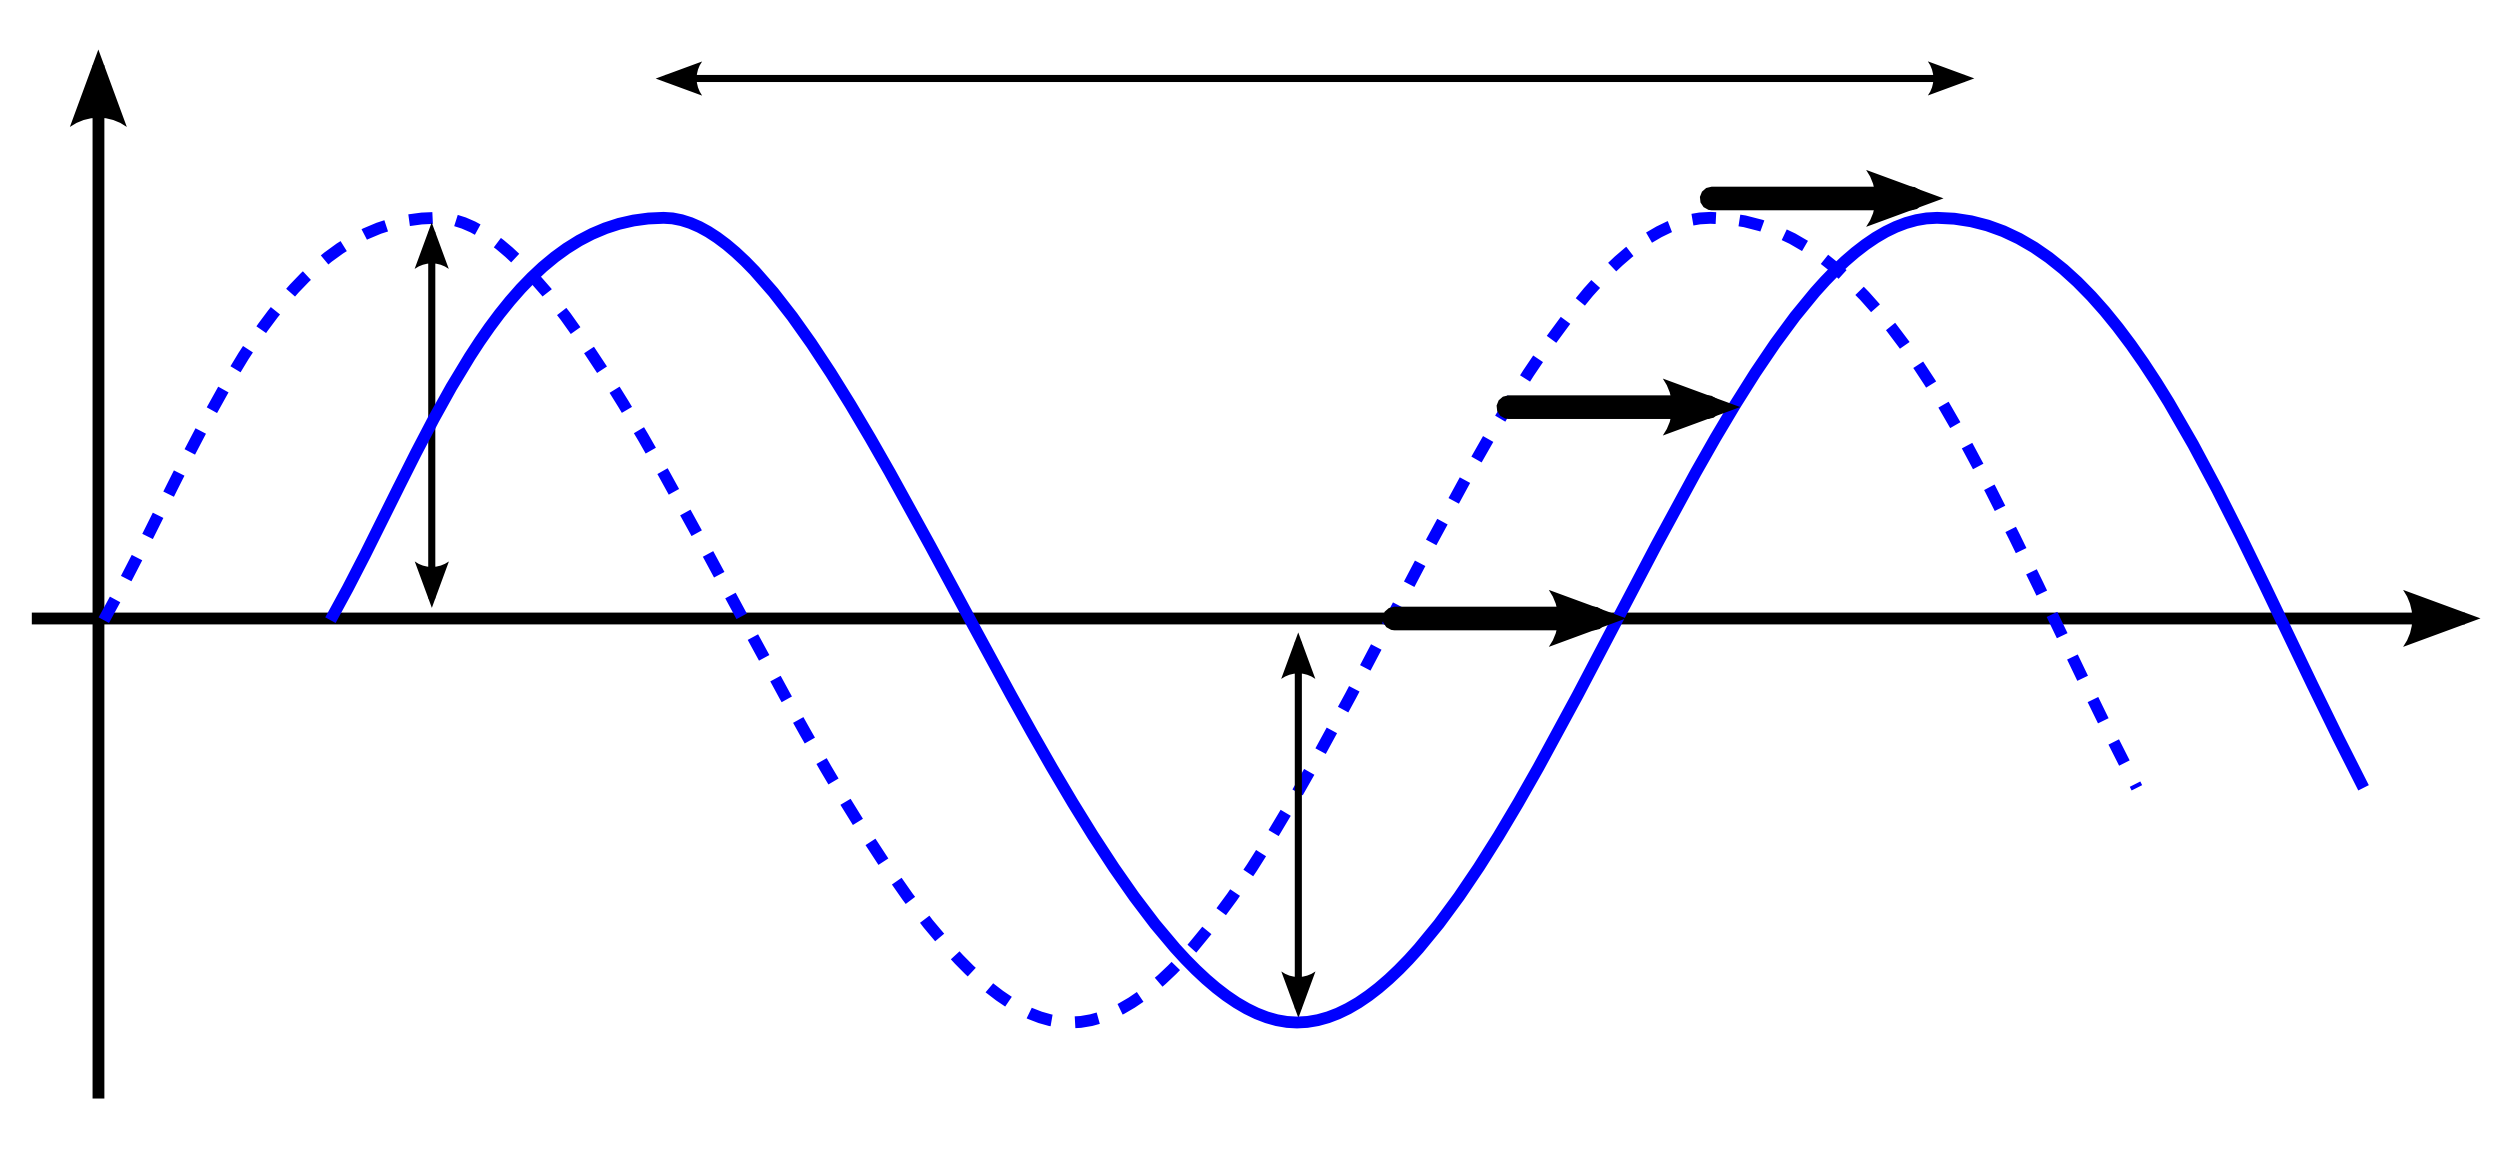
\includegraphics[width=60mm]{mode_normal.png}}
	\put(27, 27){$\lambda = 2\pi/k$}
	\put(8, 18){$|A|$}
	\put(33, 8){$|A|$}
	\put(36.5, 15){$c$}
	\put(62, 15){%
		\begin{minipage}{55mm} 
			\begin{itemize}
			\item
				$A$ : amplitude de pression 
				
				($\underline A $ amplitude complexe)
			\item
				$k = 2\pi/\lambda$ : nombre d'onde (en rad/m)
			\item
				$\lambda = 2\pi/k$ : longueur d'onde
			\item
				$\omega = 2 \pi /T$ : pulsation (en rad/s)
			\item 
				$f = 1/T = \omega/2 \pi$ : fréquence (en Hz)		
			\item
				$T = 2 \pi/\omega $ : période (en s)	
			\item
				$c = \omega/k$ : vitesse de phase (ou célérité)
			\end{itemize}
		\end{minipage}}
\end{picture}

\pause
La perturbation de vitesse associée s'écrit:
$$
	{\color{red}  u'(x, t)  = \frac{A}{\rho c_0}  \cos ( kx -\omega t + \varphi_A) } 
	$$


\pause 

\smallskip

{\color{blue} 
{\scriptsize 
Illustration multimédia :
\begin{verbatim}
http://www.animations.physics.unsw.edu.au/jw/travelling_sine_wave.htm
\end{verbatim}
}

 Illustrations avec le programme \verb| wavesimulator.m |
}


%medskip

%En injectant cette forme de solution dans l'eq. de Helmholtz, on obtient directement : $c = c_0$. 


%La célérité des ondes acoustiques est donc la même pour toutes les longueurs d'ondes (et toutes les fréquences).


%\medskip

%Les ondes sont acoustiques sont dites \textcolor{vert}{non dispersives} : 
%les sons graves se propagent donc à la même vitesse que les sons aigus\ldots

%\medskip

%\textcolor{gris}{
%Remarque  : la situation est différente pour les ondes de surface (vagues) 
%qui sont dispersives, les ondes de grande longueur d'onde se propagent plus vite que les ondes de petite longueur d'onde (cf programme M1).
%}



%\vspace{39mm}

\end{frame}

\subsubsection{Ondes stationnaires}
\begin{frame}[fragile]{Solution d'onde stationnaire harmonique}

\small

\bigskip

La superposition linéaire de deux ondes progressives monochromatiques de même amplitude conduit à une solution appelée
{\em onde stationnaire }.

\medskip
Cette solution peut s'écrire sous la forme : 
$$
p'(x,t) = A \left( \cos (kx - \omega t) + \cos ( kx + \omega t) \right) = 2 A \cos k x \cos \omega t
$$
$$
u'(x,t) = (\rho_0 c_0)^{-1} A \left( \cos (kx - \omega t) - \cos ( kx + \omega t)  \right) = \frac{2 A}{\rho_0 c_0} 
\sin k x \sin \omega t
$$

Cette situation se rencontre en particulier lors de la réflexion d'une onde progressive sur une extrémité fermée ou idéalement ouverte.

\bigskip

 
{\color{blue} 

 Illustrations avec le programme \verb| wavesimulator.m |

 Illustration multimédia :
{\scriptsize
\begin{verbatim}
http://newt.phys.unsw.edu.au/jw/strings.html
\end{verbatim}
}

}
\pause
\medskip

\begin{itemize}

\item Dans le cas d'une extrémité fermée, celle-ci est un noeud de vitesse (position où $u'=0 \quad \forall t$)  et un ventre de pression (position où $p'$ est extrémal).

\pause
\medskip

\item  Dans le cas d'une extrémité (idéalement) ouverte, celle-ci est un noeud de pression (position où $p'=0 \quad \forall t$)  et un ventre de vitesse (position où $u'$ est extrémal).


\item { \color{vert} Remarque : dans le cas d'un tuyau ouvert, une modélisation plus fine montre que le noeud de pression est en réalité à une distance $\Delta$
de l'extrémité du tuyau, où $\Delta$ est une "correction de longueur" donnée par 
 $\Delta \approx 0.61 D$ où $D$ est le diamètre du tuyau.
%L'onde se réfléchit donc (en changeant de signe) à la position $x=\Delta$.
}

\end{itemize}

\medskip

Application : on retrouve une seconde démonstration des fréquences fondamentales des tuyaux de flûte et de clarinette (TD).

\vspace{39mm}

\end{frame}

%==========================================================================================
\subsection{Energie et intensité acoustiques}
%=========================================================================================

%-----------------------------------------------------------------------------------------
\subsubsection{Equation de l'énergie cinétique}
%-----------------------------------------------------------------------------------------
\begin{frame}{Equation de l'énergie cinétique}
%-----------------------------------------------------------------------------------------

\small


Considérons a nouveau le bilan local d'énergie cinétique (cf. annexe A.3)



\begin{equation}
		\rho \ddt{} \frac{ |\vec{u}|^2}{2} 
		=   - \gradient p \cdot {\vec u} + \vec{u} \cdot \divergence ( \mytensor{\tau} )
		%\label{eq:bilan_local_lagrangien_qdm}
\end{equation}

Sous les hypothèses de l'acoustique linéaire, celui-ci peut s'écrire :

\begin{equation}
		 \dpdt{} \left( \rho_0 \frac{u'^2}{2} \right)
		 = - \divergence( p' {\vec u}' ) + p' \divergence( {\vec u}' )  
		%\label{eq:bilan_local_lagrangien_qdm}
\end{equation}


\pause

\begin{itemize}
\item
	Le premier terme correspond aux taux de variation de l'énergie cinétique volumique $e_c$.
\item
	Le deuxième terme s'interprète comme la {\em puissance extérieure des forces de pression} par unité de volume
\item
 	Le troisième correspond à {\em puissance intérieure des efforts des forces de pression} par unité de volume.

	En utilisant l'équation de la masse ce terme peut s'écrire	
	\[
		p' \divergence ( \myvec{u}') = - \frac{p'}{\rho_0} \dpdt{\rho'}  = -\frac{1}{ \rho_0 c_0^2} p'  \dpdt{p'}  = -\dpdt{e_p}
	\]
	où $e_p =  \frac{p'^2}{2 \rho_0 c_0^2}$ désigne une énergie potentielle associée à la pression acoustique.
\end{itemize}

\pause
%L'équation de l'énergie cinétique a donc pour expression
%\[
%	\color{vert}
%	\dpdt{} \left(e_c+e_p \right) = -\dpdx{}(p'u')  \]

\vspace{0mm}

\end{frame}


%-----------------------------------------------------------------------------------------
\subsubsection{Equation de l'énergie acoustique}
%-----------------------------------------------------------------------------------------
\begin{frame}{Equation de l'énergie acoustique}
%-----------------------------------------------------------------------------------------

\small

En introduisant l'\textcolor{vert}{énergie acoustique} par unité de volume
\[
	\color{vert}
	e_a = e_c + e_p = \frac{1}{2} \rho_0 u'^2 + \frac{1}{2\rho_0 c_0^2} p'^2
\]
\pause
et le vecteur \textcolor{blue}{intensité acoustique} 
\[
	\color{blue}
	\vec{I} = p' \vec{u}'
\]
\pause
le bilan local d'énergie mécanique s'écrit alors
\[
	\color{red}
	\dpdt{e_a} = - \divergence (\vec{I})	
\]

\pause

En intégrant sur un volume de contrôle $\Omega$ on obtient :
\[
\color{red}
\dpdt{}  \left[ \iiint_{\Omega} e_a dV \right] = - \oint_{\partial \Omega } \vec{I} \cdot \vec{n} dS. 
\]

\pause
Le vecteur $\vec {I}$ s'inteprète donc comme un {\em flux d'énergie acoustique} transporté (ou "rayonné") par les ondes. 


\end{frame}

\begin{frame}{flux d'énergie : cas des ondes planes progressives sinusoïdales}
\small
%\textbf{Cas d'une onde plane :} \medskip

Considérons un domaine occupé par deux ondes planes de vitesse $+c_0$ et $-c_0$ et 
d'amplitude respective $A$ et $B$ :
 
$$
p'(x,t) = A \cos (k x - \omega t) + B \cos (kx + \omega t) 
$$
$$
u'(x,t) = \frac{A}{\rho c_0}  \cos (k x - \omega t) - \frac{B}{\rho c_0} \cos (kx + \omega t)
$$

\pause
Alors on montre que :

\begin{itemize}
\item l'énergie acoustique {\em moyenne } $\overline{e_a} = \frac{1}{T} (\int_0^T e_a dt)$ vaut :
$$
\color{red} \overline{e_a} = \frac{A^2}{2 \rho c_0^2}  +  \frac{B^2}{2 \rho c_0^2} \equiv e_{a,A} + e_{a,B}
$$

(on note au passage que pour chacune des ondes les valeurs moyennes 
de l'énergie cinétique et potentielles sont égales ; en accord avec le principe de l'équipartition de l'énergie !)

\pause 
\item L'intensité acoustique moyenne vaut $\overline{ \vec{ I}} = \overline{I}_x \vec e_x$ avec :
  
$$
\color{red} \overline{I}_x = \frac{A^2}{2 \rho c_0}  -  \frac{B^2}{2 \rho c_0} 
\equiv \overline{I}_{x,A}  +  \overline{I}_{x,B} 
%\equiv  e_{a,A} c_0 -  e_{a,B} c_0
$$
\end{itemize}

Interprétation : on a $ \overline{I}_{x,A} =+ c_0 \cdot e_{a,A}   $ et $ \overline{I}_{x,B} =- c_0 \cdot e_{a,B}   $

pour chacune des ondes, le flux d'énergie est égal à la densité d'énergie multiplié par la vitesse de l'onde.

$c_0$ est donc {\em la vitesse de propagation de l'énergie.}


\pause

Remarque : pour une onde stationnaire ($A$ = $B$) le flux d'énergie net est nul ! 

($\overline{I}_x = 0$)
 


\vspace{0mm}
\end{frame}


%-----------------------------------------------------------------------------------------

\subsection{Réflexion et transmission sur une discontinuité}
%-----------------------------------------------------------------------------------------
\begin{frame}{Réflexion et transmission sur une discontinuité}

\small

Exercice complémentaire (correction sur moodle)

On étudie la propagation d'ondes dans un milieu présentant une discontinuité :

$$
(x<0 ) : \quad \rho_0 = \rho_1 ; c_0 = c_1 ; \quad \qquad (x>0 ) : \quad  \rho_0 = \rho_2 ; c_0 = c_2
$$

On suppose que le champ de pression est donné par une loi de la forme suivante :
\begin{equation}
p'(x,t) = \left\{ \begin{array}{ll} 
A \cos (k_1 x - \omega t) + B \cos(-k_1 x - \omega t) & \quad ( \mbox{ pour }  x<0) \\
C \cos (k_2 x - \omega t) & \quad ( \mbox{ pour }  x>0) 
\end{array}
\right.
\label{eq:ABC}
\end{equation}


Montrez que les coefficients de réflexion et de transmission (en intensité acoustique) sont donnés par :

\begin{equation}
R = \frac{|\overline{I_{x,B}}|}{|\overline{I_{x,A}}|} =   \frac{|B|^2/\rho_1 c_1}{|A|^2/\rho_1 c_1} = \left(\frac{\rho_1 c_1 - \rho_2 c_2}{\rho_1 c_1 + \rho_2 c_2}\right)^2,
\quad
T =  \frac{|\overline{I_{x,C}}|}{|\overline{I_{x,A}}|} =  \frac{|C|^2/\rho_2 c_2}{|A|^2/ \rho_1 c_1}    = \frac{4 \rho_1 c_1\rho_2 c_2}{(\rho_1 c_1 + \rho_2 c_2)^2}.
\label{eq:RT}
\end{equation}

\pause

Application numérique : entre l'eau et l'air $T = 0.001  \equiv -30 db$. Très mauvais !

\pause

La transmission peut être augmentée avec un dispositif mécanique "adaptateur d'impédance" dont un très bel exemple est constitué par les osselets de l'oreille moyenne.

\begin{figure}
$$
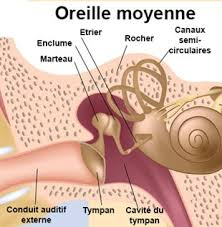
\includegraphics[width=.25\linewidth]{OreilleMoyenne.jpg}
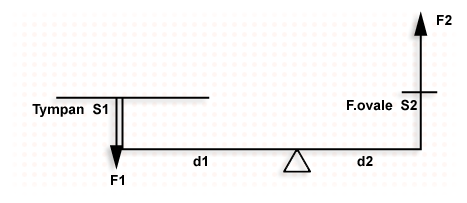
\includegraphics[width=.25\linewidth]{ModeleOreille.png}
$$
\caption{$(a)$ physiologie de l'oreille et $(b)$ Modèle mécanique simplifié des osselets de l'oreille moyenne.}
\end{figure}


\end{frame}



%-----------------------------------------------------------------------------------------
\subsection{Ondes sphériques}
%-----------------------------------------------------------------------------------------
\begin{frame}{Ondes sphériques}
%-----------------------------------------------------------------------------------------

Considérons des ondes décrites en coordonnées sphériques sous la forme $p' = p'(r,t)$ ; 
$\vec{u}'  = u(r,t) \vec{e}_r$.

En utilisant l'expression de l'opérateur Laplacien en coordonnées sphériques, l'équation de Helmholtz s'écrit :

\begin{equation}
	\color{vert}
	\ddpdt{p'} = c_0^2 \nabla^2 p' \equiv \frac{1}{r} \frac{\partial^2}{\partial r^2}\left(r p'\right)
\end{equation}

La solution générale peut s'écrire sous la forme :
$$
p'(r,t) = \frac{f(r-c_0 t)}{r} +  \frac{f(r+c_0t)}{r} 
$$

On reconnait une onde divergente et une onde convergente.


\end{frame}

\begin{frame}{Ondes sphérique : étude de l'onde divergente}
%-----------------------------------------------------------------------------------------
\small

Considérons la solution d'onde sphérique divergente définie par 
$$
p'(r,t) = \frac{f(r-c_0 t)}{r}.
$$

A partir des équations du mouvement on montre que le champ de vitesse associé est donné par $\vec{u}'  = u'(r,t) \vec{e}_r$ avec :

$$
u'(r,t) = \frac{1}{\rho_0 c_0} \left( \frac{f(r-ct)}{r} - \frac{F(r-ct)}{r^2} \right) \quad \mbox{ où } F(r') = \int f(r') d r'.   
$$

Le premier terme est dominant en champ lointain. En ne retenant que ce terme, l'énergie acoustique volumique et l'intensité acoustique sont données par :

$$
\overline{e_{ac}} = \frac{\rho u'^2}{2} + \frac{p'^2}{2 \rho_0 c_0^2} = 
\frac{\overline{f(r-ct)^2}}{\rho_0 c_0^2}
\frac{1}{r^2} 
$$

$$
\overline{\vec{I}} = \overline{p' \vec {u'} } = c_0 \overline{e_{ac}} \vec{e}_r
$$

On constate que l'intensité acoustique (flux surfacique d'énergie acoustique) décroit en $r^{-2}$.

(le flux total $ \int_S \overline{\vec{I}} \cdot \vec{n}  dS$ 
sur une sphère $S$ de rayon $r$ est constant, logique !)




\end{frame}


%-----------------------------------------------------------------------------------------
\begin{frame}{Réflexion sur la pointe d'un tuyau conique}
%-----------------------------------------------------------------------------------------

Considérons une situation correspondant à une onde divergente monochromatique d'amplitude $A$ et une onde convergente monochromatique d'amplitude $B$ :

$$
p'(r,t) =    \frac{B e^{i(kr +\omega t)}}{r} + \frac{A e^{i(kr -\omega t)}}{r} 
$$

La pression $p'(r,t)$ doit rester finie en $r=0$.

Ceci conduit à la condition $A=-B$.

\medskip

Conclusion : dans un tuyau conique, une onde (décrite en coordonnées sphériques) se réfléchit sur la pointe (fermée) en gardant changeant de signe !

\medskip

Conséquence : un tuyau conique (hautbois) a une fréquence fondamentale deux fois plus haute que celle d'un tuyau cylindrique fermé (clarinette). 

Le hautbois sonne donc une octave plus haut que la clarinette !



\end{frame}

\begin{frame}[fragile]{Illustrations multimedia}

\small
Ondes progressive (impulsion)

{\scriptsize
\begin{verbatim}
http://www.animations.physics.unsw.edu.au/jw/waves_superposition_reflection.htm#travelling
\end{verbatim}
}

Onde progressive sinusoidale

{\scriptsize
\begin{verbatim}
http://www.animations.physics.unsw.edu.au/jw/travelling_sine_wave.htm
\end{verbatim}
}


Reflexion sur une discontinuité (ondes sur une corde)

{\scriptsize
\begin{verbatim}
http://www.animations.physics.unsw.edu.au/jw/waves_superposition_reflection.htm#densities
\end{verbatim}
}

Flutes et clarinettes
{\scriptsize
\begin{verbatim}
http://newt.phys.unsw.edu.au/jw/flutes.v.clarinets.html
\end{verbatim}
}

Un bon point de départ pour en savoir plus :

{\scriptsize
\begin{verbatim}
http://www.editions.polytechnique.fr/files/pdf/EXT_0840_2.pdf
\end{verbatim}
}

\end{frame}


